%\documentclass[rnd]{mas_proposal}
\documentclass[thesis]{mas_proposal}

\usepackage[utf8]{inputenc}
\usepackage{amsmath}
\usepackage{amsfonts}
\usepackage{amssymb}
\usepackage{graphicx}

\usepackage{xcolor}
\usepackage{listings}
\usepackage{caption}
\DeclareCaptionFont{white}{\color{white}}
\DeclareCaptionFormat{listing}{%
	\parbox{\textwidth}{\colorbox{gray}{\parbox{\textwidth}{#1#2#3}}\vskip-4pt}}
\captionsetup[lstlisting]{format=listing,labelfont=white,textfont=white}
\lstset{frame=lrb,xleftmargin=\fboxsep,xrightmargin=-\fboxsep}

\lstset{
	% numbers=left,
	breaklines=true,
	% backgroundcolor=\color{light-gray},
	tabsize=4,
	% basicstyle=\ttfamily,
	literate={\ \ }{{\ }}1	
}

\title{Project Proposal Title}
\author{Abhishek Padalkar}
\supervisors{First Supervisor\\Alex Mitrevsky \\ Third Supervisor}
\date{Month 20XX}

% \thirdpartylogo{path/to/your/image}

\begin{document}

\maketitle

\pagestyle{plain}

\chapter{Introduction}
Most of the real world robotic manipulation task present the need for compliant manipulation, where robot needs to respond to the contact forces while executing the task. Classical planning and control algorithm fail to perform satisfactorily due to the lack of precise model of contact forces and high computational complexity. Various approaches have been proposed to learn compliant manipulation skills with help of Reinforcement Learning (RL). RL, in theory, is very promising when it comes to learn intelligent behaviors in complex environment with high dimensions. But it requires high number of interactions with environment. In model free reinforcement learning, a agent learns the skills by exploring the environment and adopting the parameters which governs the trajectory of the agent in the environment. Learning all the parameters of the policy can be computationally very expensive and might require large number of interactions with the environment. Application of RL to robotics is limited by above reason because large number trials causes wear and tear in mechanical parts and even damage to robot and the environment apart from being time consuming. Model based RL provide the solution to the problem of required high number of interactions with the environment by modeling some part of environment and motions policy. 

On the other hand, task specification approaches like iTasc rely on instantaneous task specification in task frame where constraint on motion are specified in each direction. Such approaches are more practical because of less number of robot interactions and deterministic nature. But some parameters in this case need to be tuned manually which is tedious task and require number of human interventions. 
Kalakrishnan et. al. in \cite{kalakrishnan2011learning} propose a control algorithm by joint RL with intelligent control which learns force policy to open door on top of the specified motion for unlatching and opening opening operation.
We propose to extend above mentioned work by using task specification like iTask and using RL for searching parameters good enough for executing the task. Our approach combines the features from model based manipulation solutions and RL. We propose to bring together the feature of deterministic solution from model based control solutions and self learning capability from RL in one solution.  
\begin{itemize}
	\item ItaSc and limitations
	\item RL and limitations
	\item model based RL
	\item propose the solution
\end{itemize}
\begin{itemize}
	\item In model free reinforcement learning, an agent learns the skills by exploring the environment and adopting the parameters which governs the trajectory of the agent in the environment.
	\item Learning all the parameters of the policy can be computationally very expensive and might require large number of interactions with the environment.
	\item Application of RL to robotics is limited by above reason because large number trials causes wear and tear in mechanical parts and even damage to robot and the environment apart from being time consuming. 
	\item If we can model the environment and constraints on the motion of the robot, we can drastically reduce the number of parameters to be learn to achieve the task.
	\item Use of reinforcement learning to learn these reduced number of parameters can result in near optimal policy for achieving the task.
	\item 
\end{itemize}
\begin{itemize}
    \item Manipulation tasks imply complex contact interactions with an unstructured environment and require a controller that is able to handle force interactions in a meaningful way \cite{kalakrishnan2011learning}.
    \item planning algorithms would require precise dynamics models of the resulting contact interactions. These models are usually unavailable, or so im- precise that the generated plans are unusable\cite{kalakrishnan2011learning}.
    \item A lot of times humans manipulate objects by dragging them on the surface from one place to another. This saves energy because we don't have to lift and place the object. Robots can do the same. 
    \begin{itemize}
    	\item Object manipulation with less energy.
    	\item Pushing objects away to reach for another object in cluttered space.
    \end{itemize}
\end{itemize}

\section{Problem Statement}
\begin{itemize}
    \item We propose to create a framework based on task specification and model based reinforcement learning to solve the problem of compliant manipulation for given task in deterministic manner with fewer number of interactions with environment.
    \item We will evaluate our approach based by learning a demo task of opening door. We will evaluate it on the basis of number of interactions needed with environment, deterministic .
\end{itemize}


\chapter{Related Work}
\section{Task specification}
In industrial settings, task are usually specified in the form of sequence of primitives \cite{leidner2017cognitive}. These primitives mostly contain point-to-point motion, motion to some default configuration and basic curves. For example, following script taken from FRI interface examples shows the example motion primitives as shown in listing \ref{KRL-sample}. Though this kind of task specification works in controlled industrial environment, it leaves very little scope for external sensory feedback and the task needs to specified in terms of positional goals.

\begin{lstlisting}[label=KRL-sample,caption=KRL code]
INI
PTP HOME ; go to HOME joint configuration
LIN P1   ; linear motion to point P1
LIN P2	 ; linear motion to point P2
\end{lstlisting}

In \cite{leidner2017cognitive}, Leidner presented a representation in the form of action templates describing robot action using symbolic representations and geometric process model as shown in listing \ref{a-template}.  Symbolic representation of the task in PDDL allows classical planners to consider the action in the high level abstract task plan and geometric representation of the task specifies the sequence of low level movement sequences needed to complete the action. Here, geometric representation only specifies discrete motion primitives and not the parametric representation of the motion primitives. Actual parameterization and control is left to low level control module.   

\begin{lstlisting}[label=a-template,caption=Action Template: \_object.pick]
I Symbolic Representation 

'''
(:action _object.pick: 
:parameters (?o - _object ?m - _manipulator ?s - _surface) 
:precondition (and(free ?m) (on ?o ?s)) 
:effect (and(bound ?o ?m) (not(free ?m)) (not(on ?o ?s)))
) 
''' 

II Geometric Representation

def pick(self, manipulator, surface):
''' approach, grasp, and lift an object from a surface '''

graspset = odb.get_property(self.type, 'graspset', manipulator) 
for grasp_candidate in graspset: 
if grasp_candidate in self.history: 
continue
self.history.append(candidate) 
grasp = grasp_candidate 
break

if grasp is None: 
raise RuntimeError('no more alternatives')
else: 
self.grasp = grasp
operations = [
('move_hand', manipulator, g.approach_grasp), 
('plan_to_frame', manipulator, g.approach_frame, self.frame), ('plan_to_frame', manipulator, g.grasp_frame, self.frame), 
('bind', manipulator, self.name), 
('move_hand', manipulator, g.pre_grasp), 
('move_hand', manipulator, g.grasp), 
('move_straight', manipulator, txyz(0, 0, 0.1))
] 
return operations
\end{lstlisting}

In \cite{mason1981compliance}, Mason et. al. presented the idea behind \textit{Task Frame Formalization - TFF} for representing compliant task. Using hybrid control, various control modes are assigned to each axis of the \textit{task frame} or \textit{compliance frame}\cite{nagele2018prototype}. Listing \ref{tff} shows Open Door task taken from \cite{bruyninckx1996specification}. This framework doesn't consider the specification of task or motion quality related parameters like velocity damping or instantaneous sensory inputs. It also specify action to executed \textit{compliantly} but does not specify the how? 

\begin{lstlisting}[label=tff,caption=Task Specification using TFF: Open Door]
move compliantly {
	with task frame directions
	xt: force 0 N
	yt: force 0 N
	zt: velocity v mm/sec
	axt: force 0 Nmm
	ayt: force 0 Nmm
	azt: force 0 Nmm
} until distance > d mm 
\end{lstlisting}


iTaSC developed in \cite{DeSchutter-ijrr2007, DecreBruyninckxDeSchutter2013, decre09}, synthesizes control inputs based on provided task space constraints. It formulates a optimization problem considering provided constraints in the environment. In case of conflicting constraints, constraints are weighted in the optimization problem.  


\section{Door Opening}

Opening door is one the most important task for service and rescue robots. Number of studies have been conducted to investigate this challenging problem using different techniques. Number of approaches rely on detail geometric modeling of the door and analytical trajectory generation. Nagatani et.al. \cite{nagatani1995experiment} presented an early approach for opening door by modeling the geometry of the door and then synthesizing trajectory to open door by considering geometrical constraints. To cope with the errors in position control of the early days manipulator used in the experiment, they used a force torque sensor module to achieve compliance with the environment. But this approach highly relies on correct geometric model and accurate execution of designed trajectories.

Approaches presented in \cite{levihn2014using,karayiannidis2012adaptive,niemeyer1997simple} use adaptive control algorithms which synthesize the motion by identifying the environmental constraints. In \cite{karayiannidis2012adaptive}, authors proposed to find the radial direction based on force and torque readings. Door is opened by applying velocity in radial direction. This method is prone to failure in case of uncertain grasp position. Also it considers only the case where door is already unlatched. 

Some of the methods for door opening motor primitives like Dynamic motion primitives for generating trajectories for opening door. Disadvantage of these approaches is that we need to know the goal pose to generate trajectory hence it confines the condition of completing the task to achieving a goal pose. 


\chapter{Proposed Solution}

We plan to solve a compliant manipulation task by providing model of the environment and then tuning the task parameters with the help of re-reinforcement learning.

Examples of task modeling: 

\begin{lstlisting}[label=open_door_ts,caption=Task specification for opening door]
open_door
{
	f_x = f($\Theta$(environment, robot, task))
	v_y = $v$
	max_acc = $a_{max}$
	max_dec = $a_{dec}$
}until(f(...))

\end{lstlisting}


\begin{lstlisting}[label=assist_ts,caption=Task specification for assisting human]

assist_human_to_carry
{
	f_x = f($\Theta$(environment, robot, task))
	v_x = g1(ft_sensor_measurement)
	v_y = g2(ft_sensor_measurement)
	v_z = g3(ft_sensor_measurement)
	damping_x = C1
	damping_y = C1
	damping_z = C1
}until(f2(...))

\end{lstlisting}

Above task specification has the parameters which needs to be tuned either manually or automatically. These parameters will be tuned with model based RL.

\begin{figure}[!h]
	\center{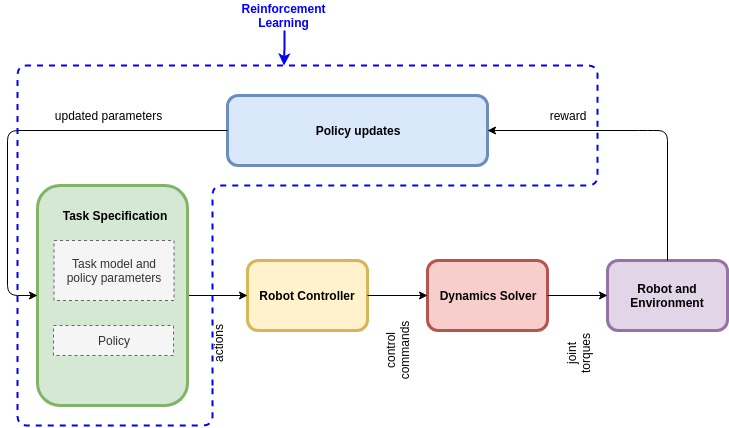
\includegraphics[width=\textwidth]
		{images/composition.png}}
	\caption{\label{fig:composition} Composition}
\end{figure}
Above figure shows the composition of the framework.
\chapter{Project Plan}

\section{Work Packages}
The bare minimum will include the following packages:
\begin{enumerate}
    \item[WP1] Literature Search
    \item[WP2] Experiments
    \item[WP3] Project Report
\end{enumerate}
Keep in mind that depending on your project, you will probably need to add work packages that are more suited to your projects.

\section{Milestones}
\begin{enumerate}
    \item[M1] Literature search
    \item[M2] Experimental setup
    \item[M3] Experimental Analysis
    \item[M4] Report submission
\end{enumerate}

\section{Project Schedule}
Include a gantt chart here. It doesn't have to be detailed, but it should include the milestones you mentioned above.
Make sure to include the writing of your report throughout the whole project, not just at the end.

\begin{figure}[h!]
    \includegraphics[width=\textwidth]{rnd_deliverable_timeline}
    \caption{}
    \label{}
\end{figure}

\section{Deliverables}
\subsection{Minimum Viable}

\begin{itemize}
    \item Survey
    \item Analysis of state of the art
    \item Simple simulated use case
    \item Demo on youBot or Jenny
\end{itemize}

\subsection{Expected}
\begin{itemize}
    \item Comparation of approaches in the robot
\end{itemize}

\subsection{Desired}
\begin{itemize}
    \item Integration to scenario
\end{itemize}


\nocite{*}

\bibliographystyle{plainnat} % Use the plainnat bibliography style
\bibliography{bibliography.bib} % Use the bibliography.bib file as the source of references




\end{document}
